% !TEX encoding = MacOSRoman
\documentclass[12pt,a4paper,english]{article}

% Note that you must choose either Finnish or English here and there in this
% file.
% Other options for document class
  % ,twoside,openright   % If printing on both sides (>80 pages)
  % ,twocolumn           % Can be used in lab reports, not in theses

% Ensure the correct Pdf size (not needed in all environments)
\special{papersize=210mm,297mm}

\usepackage[utf8]{inputenc}
\usepackage[T1]{fontenc}
\usepackage{hyperref}
\usepackage{amsfonts}
\usepackage{textcomp}
\usepackage{listings}
\usepackage{graphicx}
\usepackage{numprint}
\usepackage{subfigure}
\usepackage{tikz}
\usetikzlibrary{shapes.geometric, arrows}
\usepackage{setspace}
\usepackage{termlist}
\usepackage{amsmath}
\usepackage{amssymb}
\usepackage{amsthm}
\usepackage{bm}

%new commands
\newcommand\todo[1]{{\color{red}!!!TODO: #1}}
\DeclareMathOperator{\tr}{\mathrm{tr}}

\author{Jordi Anguera\thanks{Autonomous University of Barcelona, Spain} \and Leevi Annala\thanks{University of Jyväskylä, Finland} \and Stefan Dimitrijevic\thanks{University of Novi Sad, Serbia} \and Patricia Pauli\thanks{Technical University of Darmstadt, Germany} \and Liisa-Ida Sorsa\thanks{Tampere University of Technology, Finland} \and Dimitar Trendafilov\thanks{University of Sofia ''St. Kliment Ohridski'', Bulgaria} \and Christophe Pickard\thanks{University of Grenoble Alpes and Grenoble INP, France}}
\title{Modeling effect of time delay for large network of seismic monitor} 
\date{17.7.2018}

\begin{document}
\maketitle

\begin{abstract}

\end{abstract}

\section{Introduction}

The purpose of this work is to analyze noise in a large network of seismic monitors and to extract clock drift from the noise. 

\section{Data}

Number of working connections over time (Figure \ref{fig:workingconnections}). 

\begin{figure}[ht]
  \begin{center}   
   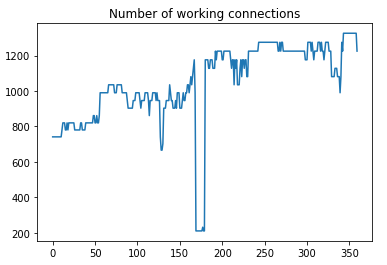
\includegraphics[width=0.7\textwidth]{working_connections.png}
  \end{center}
  \caption{The number of working connections in the network over time. }\label{fig:workingconnections}
\end{figure}

\section{Methods}

\subsection{Basic variables, the model}
We have a network of seismic monitors recording ground vibrations. The monitor records compression and decompression as discrete values -1 and 1, respectively, every second. The GPS coordinate position of each monitor in the network is known (Figure \ref{fig:monitornetwork}). 

\begin{figure}[ht]
  \begin{center}   
   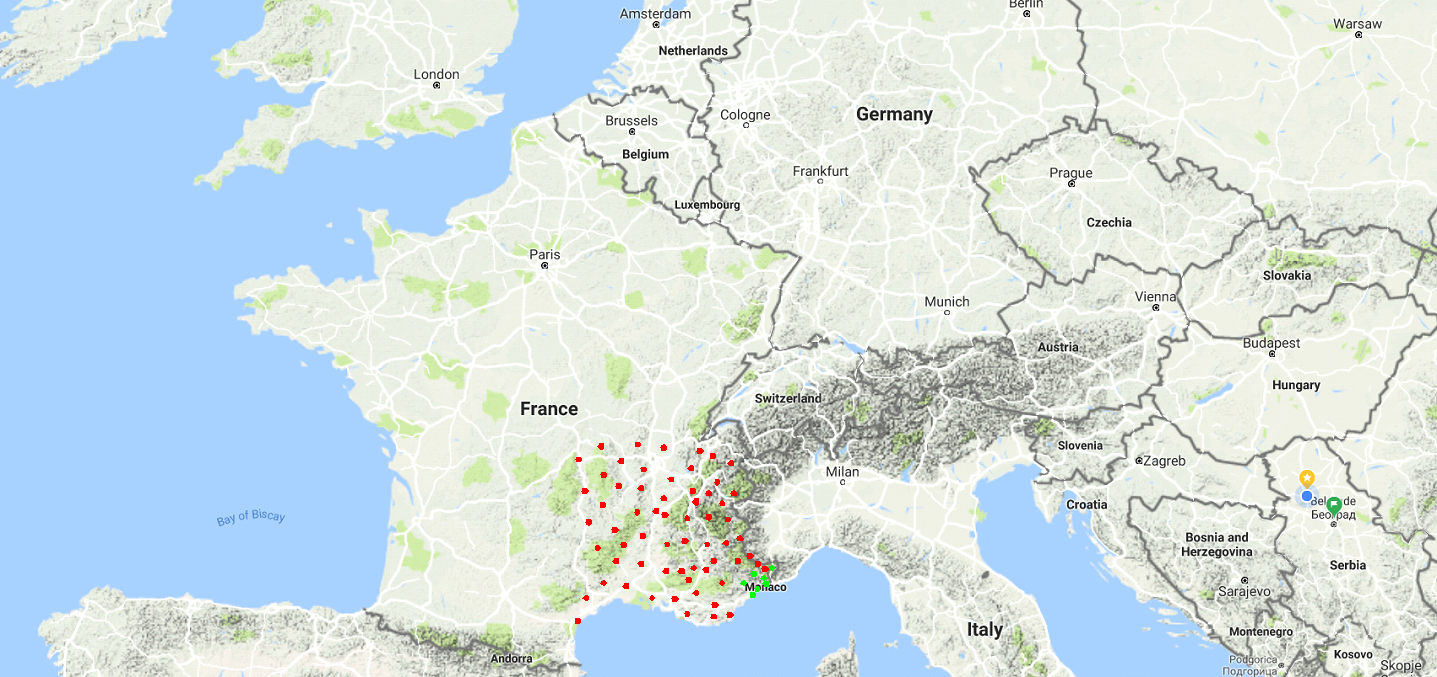
\includegraphics[width=\textwidth]{InitialStationSet.png}
  \end{center}
  \caption{The network of seismic monitors are located in the Southeast France, mostly in the regions of Provence-Alpes-C\^{o}te d'Azur and Rh\^{o}ne-Alpes. The seven stations chosen as the small test set is shown as green in the southeast part of the area.}\label{fig:monitornetwork}
\end{figure}

The network of monitors can be modelled as a complete graph. The signal of each monitor is cross-correlated with other monitor signals, finally yielding time-delay data between each monitor. The time delay between the monitors comprise information on the real time the signal travels between the monitors, the inaccuracies of the clock (time drift), and other noise affecting the measurement. 

Let $\bm{\hat{\delta}} \in \mathbb{R}^{n\times n}$ be the measured pairwise time delays of the system, $\bm{\delta}$ the actual pairwise time delays, and $\bm{\varepsilon}$ an error term including clock drift of the station's clock and other errors

\begin{equation}
\bm{\hat{\delta}}  = \bm{\delta} + \bm{\varepsilon}.
\label{eq:model}
\end{equation}
 
Each of the monitors are equipped with a clock which runs independent of others. It is synchronized via GPS system once a month and then runs independently. The drift, $\varepsilon_i$ in clock $i$ is caused by variation in the clocks oscillator.  

The position of each seismic monitor in the network is known. As the monitors are spread across a large area, it is assumed that local tremors are detected by stations that are close by, and therefore the correlations found in the pairwise cross-correlations and time delay data between them have higher likelihood to be linked. 

\subsection{Denoising model}

The computational denoising model involves weighted network estimation by the use of topological graph metrics, described in detail in \cite{Spyrou2017}. 

We have a weighted graph $\mathcal{G} = (\mathcal{V}, \mathcal{E}, \bf{\hat{\delta}}_t)$ defined by a finite set of nodes $\mathcal{V}$ with $|\mathcal{V}| = n$, a set of edges $\mathcal{E} = \{ (v_i,v_j) \in \mathcal{E} \}$, with $|\mathcal{E}| = n^2-n$ and the weighted adjacency matrix $\bm{\hat{\delta}}$ with $\delta_{ii} = 0$ for all $i$. The matrix $\bm{\hat{\delta}}$  is symmetric and describes the time delays between events in the graph, and is normalized, i.e. $\hat{\delta}_{ij}\in [0,1]$. The adjacency matrix indicates the strength of connection between nodes. Therefore, the shorter the time delay between nodes, the stronger the connection, and higher the value. 


We assume to have estimates of $M$ differentiable graph metrics of the original matrix $\delta$, i.e. $f_m(\delta) = K_m$, where $m\in\{ 1,\dots, M \}$, then we can formulate a cost function that measures the deviation of the observed weight matrix's metrics $f_m(\mathbf{\hat{\delta}}) = K_m$ 

Graph metrics are scalar functions of the weight matrix, $f(\bm{\hat{\delta}}): \mathbb{R}^{n \times n}\rightarrow \mathbb{R}$. We choose graph metrics to:
\begin{enumerate}
\item \textbf{Distance}: The distance strength of a node $i$ describes the connection strength of that node to all other nodes. The metric is calculated based on the reciprocal of distances of the node to all other nodes, $d _{ij}= 1/r_{ij}$, normalized between $[0,1]$. The higher value corresponds to nodes with short distances to all other nodes. 
\begin{equation}
d_i = \sum{d_{ij}},  
\end{equation}
with the degree derivative being:
\begin{equation}
\frac{\partial d_i}{\partial \bm{\delta}}= \mathbf{R_i}^T,
\end{equation} 

in which $R_i$ is matrix with ones at column $i$. Since $\mathbf{R}_i$ is non-zero only for column $i$ it can be computed efficiently as 

\begin{equation}
\frac{\partial d_i}{\partial \bm{\delta}_i} = \mathbf{1}_n^T, 
\end{equation} 
 
where $\bm{\delta}_i$ is the $i$th column of $\bm{\delta}$
 
\item Average neighbour degree, resilience: 

The average neighbour degree for node $i$ is given by

\end{enumerate}




%% Insert bibliography
\bibliographystyle{abbrv}  
\bibliography{references}   

\end{document}
